\documentclass[10pt,a4paper]{article}

\usepackage{xcolor}
\usepackage{geometry}
\usepackage{hyperref}
\usepackage{adjustbox}
\usepackage{fontawesome}
\usepackage{tikz}
\usepackage{makecell}
\usepackage{booktabs}% http://ctan.org/pkg/booktabs
\newcommand{\tabitem}{~~\llap{\textbullet}~~}


\usepackage[T1]{fontenc}
\usepackage[utf8]{inputenc}
\usepackage[default]{lato}

\hypersetup{
    colorlinks=true,
    linkcolor=black,
    urlcolor=black,
    pdftitle={Curriculum Vitae},
    pdfpagemode=FullScreen
}

\geometry{
    left=1cm,
    right=1cm,
    marginparwidth=6.8cm,
    marginparsep=1.2cm,
    top=1.25cm,
    bottom=1.25cm,
    footskip=2\baselineskip
}

\definecolor{star}{HTML}{deca37}
\colorlet{accent}{blue!70!black}
\colorlet{heading}{black}
\colorlet{emphasis}{black}
\colorlet{body}{black!80!white}

\newcommand*\circled[1]{\tikz[baseline=(char.base)]{
            \node[shape=circle,draw,inner sep=2pt] (char) {#1};}\,}

\newcommand{\printinfo}[2]{\mbox{\textcolor{accent}{\normalfont #1}\hspace{0.5em}#2\hspace{2em}}}

\newcommand{\emailsymbol}{\faAt}
\newcommand{\githubsymbol}{\faGithub}

\newcommand{\github}[1]{\printinfo{\githubsymbol}{#1}}
\newcommand{\email}[1]{\printinfo{\emailsymbol}{#1}}

\newcommand{\svssec}[1]{%
{\color{heading}\LARGE\bfseries\MakeUppercase{#1}}\\[-1ex]%
  {\color{heading}\rule{\linewidth}{1.5pt}\par}\medskip}

\newcommand{\cvtag}[1]{%
  \tikz[baseline]\node[anchor=base,draw=body!30,rounded corners,inner xsep=1ex,inner ysep =0.75ex,text height=1.5ex,text depth=.25ex]{#1};
}

\begin{document}

\pagenumbering{gobble}

\raggedright\color{black}%
    {\Huge\bfseries\MakeUppercase{Ferrulli Massimiliano}\par}

\vspace{0.4cm}

\faLinkedinSquare{\href{https://www.linkedin.com/in/massimiliano-ferrulli-ab7507223/}{Linkedin Profile}} \hspace{0.7cm}
\github{\href{https://github.com/MassimilianoCEZ/}{github.com/MassimilianoCEZ}}%
\email{\href{mailto:maxferrulli8@gmail.com}{maxferrulli8@gmail.com}}




\begin{minipage}[t]{0.45\textwidth}
\svssec{EDUCATION}

%{\large\circled{1}\color{accent}Scuola Primaria Alessandro Manzoni}\par
%\makebox[0.75cm]{}\makecell[l]{%
%\textit{Elementary School} \\
%\faCalendar\, 2010 -- 2014 \\
%\faMapMarker\, Lavena Ponte Tresa, Varese%
%}
%
%
%
%{\large\circled{2}\color{accent}Scuola Primaria di Caslano}\par
%\makebox[0.75cm]{}\makecell[l]{%
%\textit{Elementary School} \\
%\faCalendar\, 2014 -- 2015 \\
%\faMapMarker\, Caslano, Ticino%
%}



{\large\circled{1}\color{accent}Scuola Media Agno}\par
\makebox[0.75cm]{}\makecell[l]{%
\textit{Middle School} \\
\faCalendar\, 2015 -- 2019 \\
\faMapMarker\, Agno, Ticino%
}

\vspace{0.25cm}

{\large\circled{2}\color{accent}Liceo Lugano 2 Savosa}\par
\makebox[0.75cm]{}\makecell[l]{%
\textit{OS FAM} \\
\faCalendar\, 2019 -- 2023 \\
\faMapMarker\, Savosa, Ticino \\
\tabitem Attestato di maturità liceale
}

\vspace{0.5cm}


{\large\circled{1}\color{accent}EPFL}\par
\makebox[0.75cm]{}\makecell[l]{%
\textit{Politechnique School} \\
\faCalendar\, 2023 -- present \\
\faMapMarker\, Lausanne, Vaud \\
\tabitem Bechelore in Microtechnique
}

\vspace{0.25cm}

\svssec{Events}


{\large\color{accent}Maturaarbeit in quantum mechanics}\par
\makebox[0.75cm]{}\makecell[l]{%
\faCalendar\, 2022-2023 \\
\textit{My Maturaarbeit in quantum mechanics goes over various} \\ \textit{quantum mechanics topics such as the Franck-Hertz } \\  \textit{experiment,the blackbody radiation and both time}\\
\textit{dependent and stationary Schrödinger's equations.  }  \\ \textit{This work received 6 as a mark, which is the highest } \\ \textit{mark in Ticino.  } \\
\faGithub\, \href{https://github.com/MassimilianoCEZ/LAM}{/MassimilianoCEZ/LAM}
}

\vspace{0.25cm}

{\large\color{accent} Project for the National contest Swiss Youth SJF} \par
\makebox[0.75cm]{}\makecell[l]{%
\faCalendar\, 2022-2023 \\ 
\textit{I've partecipated in the 57th edition of the national } \\ \textit{contest for Swiss Youth in science as a finalist.} \\  \textit{For this contest I tried to recreate the electron diffraction} \\ \textit{experiment setup with a low budget of roughly 10 \% } \\  \textit{of the price proposed by the manufacturing companies.}\\ \textit{The other goal is to develop a design that allows  } \\ \textit{students to recreate this experiment in their school's lab.} \\ \textit{This work has been rewarded with the mention Very Good. } \\
\faGithub\, \href{https://github.com/MassimilianoCEZ/sjf}{/MassimilianoCEZ/sjf} \hspace{0.5cm}
\faFilePdfO \, \href{https://drive.google.com/file/d/1AHKfb-wR5lkNUCVFg81OiIKSTXmxs8Fm/view?usp=share_link}{SJF certificate} \\
\faFileTextO \, \href{https://amp.tio.ch/ticino/attualita/1662494/lugano-liceo-lavoro-ricerca-nove-promesse}{tio article} \hspace{2.35cm}
\faFileTextO \, \href{https://www.rsi.ch/news/ticino-e-grigioni-e-insubria/Giovani-scienziati-ticinesi-agli-onori-16194718.html}{Rsi article} \\
}





\vspace{0.25cm}


{\large\color{accent}Lab Day at ETHz} \par
\makebox[0.75cm]{}\makecell[l]{%
\faCalendar\, 23 August 2023 \\ 
\textit{Prof. Dr. Crivelli invited me and \href{https://www.linkedin.com/in/stefano-hauswirth-214b87260/}{Stefano Hauswirth} to visit} \\ \textit{his laboratories in the ETHz campus in Hönggerberg} \\
}


\vspace{0.25cm}

{\large\color{accent}Young Talent Day} \par
\makebox[0.75cm]{}\makecell[l]{%
\faCalendar\, 4th September 2023 \\ 
\textit{The Swiss Physical Society (SPS) invited me and other  } \\ \textit{youths to the SPS Young Talent Day at the university of } \\ \textit{Basel. We visited various laboratories and attended the } \\ \textit{Blaise Pascal Symposium in onor of his 400th birthday.} \\
}


\vspace{0.25cm}






\end{minipage}\hfill\vrule depth 23cm\hfill%
\begin{minipage}[t]{0.45\textwidth}
\svssec{Personal info}

\begin{center}
\begin{tikzpicture}
	\clip (0,0) circle (2cm) node {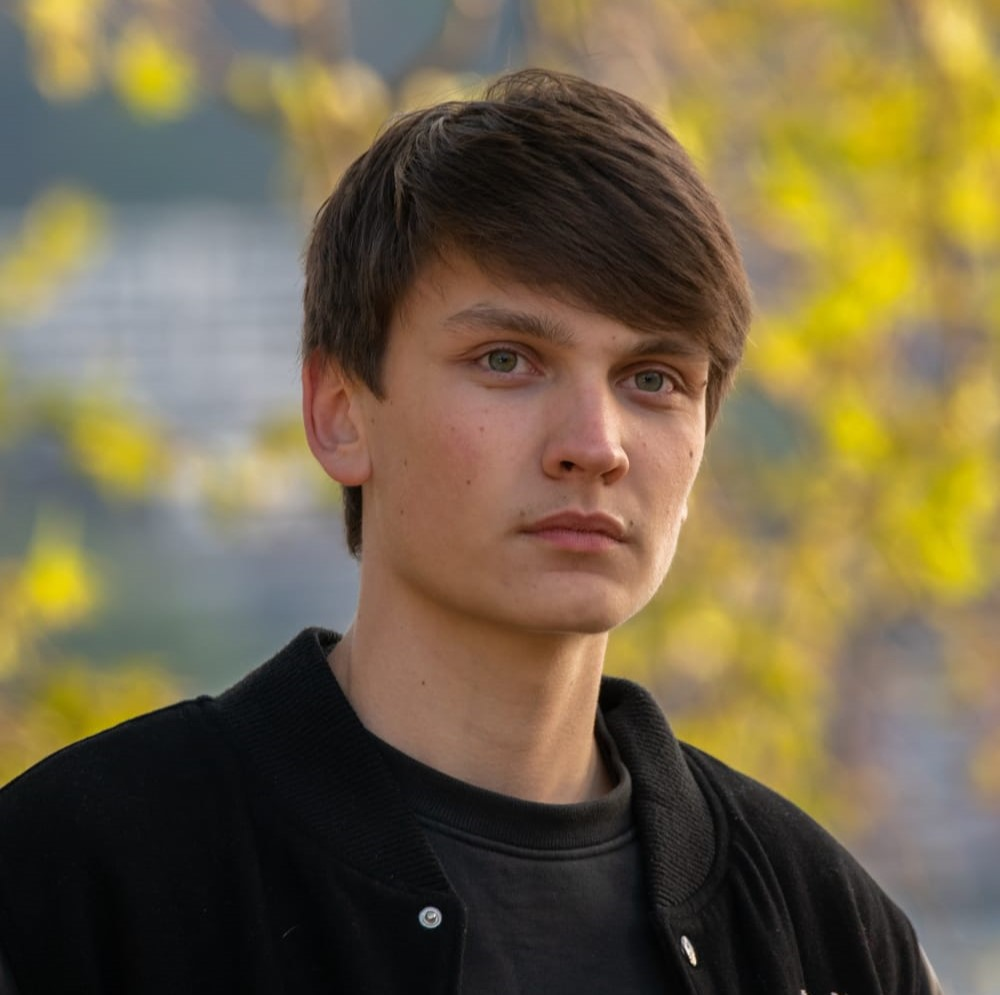
\includegraphics[width=4cm]{foto_FM2.jpg}};
\end{tikzpicture}
\end{center}

\textbf{Full name:} Ferrulli Massimiliano \\
\textbf{Date of birth:} June 8th, 2004 \\
\textbf{Nationality:} Italian

\vspace{0.5cm}

\svssec{Technologies}



\cvtag{C++}
\cvtag{Catia V5}
\cvtag{Python}
\cvtag{KiCAD}
\cvtag{Object Oriented Programming}
\cvtag{Makefile}
\cvtag{Arduino}
\cvtag{\LaTeX}
\cvtag{Solidworks}
\cvtag{Autodesk Inventor}
\cvtag{Houdini Fx}
\cvtag{Adobe After Effects} 





\vspace{0.5cm}

%% \svssec{Work Experience}
%% {\large\color{accent} Internship at Sarmap}\par
%% \makebox[0.75cm]{}\makecell[l]{%
%% \textit{Internship} \\
%% \faCalendar\, 2018, 1 day \\
%% \faMapMarker\, Monteggio  \\
%% }

\vspace{0.5cm}

\svssec{Languages}
\tabitem Italian (Native speaker, C2) \par
\tabitem English (C1) \par
\tabitem French (B2)

\vspace{0.5cm}

\svssec{Projects}

{\large\color{accent}Hand lever winch }\par
\makebox[0.75cm]{}\makecell[l]{%
\faCalendar\, 2024 \\
\textit{This is the semester project for the mechanical construction } \\ \textit{course where we had to engineer a "treuil de fôret". } \\ \textit{We went for a lever design with a planetary gearbox.} \\ \textit{More infos on my github page} \\ 
\faGithub\, \href{https://github.com/MassimilianoCEZ/Hand-lever-winch}{/MassimilianoCEZ/Hand-lever-winch}
}

\vspace{0.25cm}


{\large\color{accent} 2D simulation of a micro system in water} \par
\makebox[0.75cm]{}\makecell[l]{%
\faCalendar\, 2024\\ 
\textit{In duo we developped a 2d simulation in c++} \\ \textit{of a micro system in water. This project uses c++ 17} \\ \textit{with makefile and GTKM4 as library for the GUI} \\
\faGithub\, \href{https://github.com/MassimilianoCEZ/MicroReef}{/MassimilianoCEZ/MicroReef}
}




\vspace{0.5cm}

\svssec{Personality / interests}

I'm a curious, extrovert and determined guy. In my spare time I like to build drones, design pcbs, create cgi simulations in Houdini.
\end{minipage}

\end{document}